%documento de clase
\documentclass[a4paper,12pt]{article}

%paquetes
\usepackage[utf8]{inputenc}
\usepackage[spanish,es-tabla,es-nolayout,es-nodecimaldot]{babel}
\usepackage[total={18cm, 21cm}, top=2cm, left=2cm]{geometry}
\usepackage{amsmath, amssymb, amsfonts, latexsym}
\usepackage{graphicx}
\usepackage[x11names,table]{xcolor}
\usepackage{multicol}
\usepackage{nicefrac}
\usepackage{multirow}
\usepackage{longtable}
\usepackage{booktabs}
\usepackage{url}


%comandos
\title{inserción de gráficos}
\author{Alexis Villavicencio}
\date{\today}

%contenido
\begin{document}
\maketitle
La suluci\'{o}n a la ecuaci\'{o}n diferencial

\begin{align*}
 &\text{y}^{'}(\text{x})+2\text{y}(\text{x})=
 \begin{cases}
 1 \quad \text{ si } \, \text{ x }\in[0,3],\\
 0 \quad \text{ si } \, \text{ x } > 3;
 \end{cases}  \\
 &\text{sujeto a}
\end{align*}
\[
\text{y}(0)=0
\]

Esta dada por la función a trozos 

\begin{align*}
 \text{y}(x)=
 \begin{cases}
 \dfrac{1}{2} \big(\exp(-2\text{ x }) -1) \quad &\text{ si } \text{ x } \leq 3\\
 \\
\dfrac{1}{2} \big(\exp(-2\text{ x })- \exp(6-2\text{ x }) )  &\text{ si } \text{ x } > 3
\end{cases} 
\end{align*}
\begin{center}
 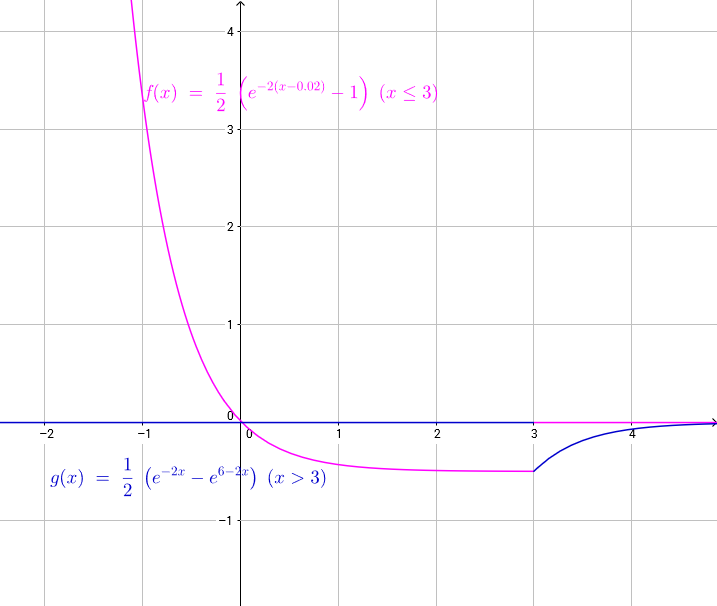
\includegraphics[scale=0.5]{figura1}
\end{center} 
 
\end{document}